\chapter{More Details on \textsc{Patus} Stencil Specifications}

In the current version, \textsc{Patus} stencil specifications\index{stencil specification} consist of $3$ parts: the size of the domain,
a $d$-dimensional grid, to the points of which the stencil is applied; a specification of the number of
time steps (sweeps) that is performed within one stencil kernel call;
and, most importantly, the ``operation'': the definition of the actual stencil expression(s), which is
applied to each point of the grid(s) over which the computation sweeps.\\
The following listing shows a skeleton of a stencil specification:
\begin{lstlisting}[language=stencil]
stencil ~\textit{name}~
{
    domainsize = (~$x_{\text{min}}$~ .. ~$x_{\text{max}}$~, ~$y_{\text{min}}$~ .. ~$y_{\text{max}}$~, ~$\dots$~);
    t_max = ~\textit{number of sweeps}~;

    operation (~\textit{grid argument and parameter declarations}~)
    {
    	~\textit{stencil expressions}~
    }
}
\end{lstlisting}

Sweeps are not programmed explicitly
in the stencil specification; the operation only contains a localized, point-wise stencil expression.
Currently, \textsc{Patus} supports Jacobi iterations, which means that the
grids which are written to are distinct in memory from the grids that are read. In the future, other types
of grid traversals, e.g., red-black Gauss-Seidel sweeps, may be supported. Given the Jacobi iteration as
structural principle, there are no loop carried dependencies within the spatial iteration over the
grid. Hence, the order in which the grid points are visited and the stencil expressions evaluated does not
matter. This fact is actually exploited by the Strategies.

Both the domain size and the number of sweeps can contain symbolic identifiers, in which case these identifiers
are added as arguments to the stencil kernel function in the generated code.
The dimensionality of the stencil is implicitly defined by the dimensionality of the domain size and the
subscripts in the stencil expressions. Currently, it is not possible to mix grids of different dimensionalities.
$x_{\text{min}}, x_{\text{max}}, \dots$ can be integer literals, identifiers, or arithmetic expressions.
\textit{Number of sweeps} can be either an integer literal or an identifier if the number of time steps has to
be controlled from outside the stencil kernel. Both minimum and maximum expressions in domain size specifications
are inclusive, i.e., the domain size $(x_{\text{min}} .. x_{\text{max}}, \dots)$ has $x_{\text{max}}-x_{\text{min}}+1$
points in $x$-direction.

There can be arbitrarily many grid arguments to the stencil
operation, depending on the application. For instance, discretizing the divergence operator, which maps vector
fields to a scalar function, might be implemented in the 3D case with three grids, which are read, and one grid
to which the result is written.
Grid arguments (in first line in the following listing) and parameter declarations (second line) have the following form:

\begin{lstlisting}[language=stencil]
~$[$~const~$]$~ ~$($~float~$|$~double~$)$~ grid ~\textit{grid name}~ ~$[$~( ~$x^{\prime}_{\text{min}}$~ .. ~$x^{\prime}_{\text{max}}$~, ~$y^{\prime}_{\text{min}}$~ .. ~$y^{\prime}_{\text{max}}$~, ~$\dots$~ )~$]$~ ~{\color{gray}$\dlsh$}~
		~$[$~[ ~\textit{number of grids}~ ]~$]$~
~$($~float~$|$~double~$)$~ param ~\textit{parameter name}~ ~$[$~[ ~\textit{array size}~ ]~$]$~
\end{lstlisting}

Both grids and parameters can either be based on single or double precision floating point data types.
If a grid is declared to be \texttt{const}, it is assumed that the values do not change in time, i.e., the
grid is read-only. The optional grid size specification after the grid name defines the size of the array
as it is allocated in memory. This is useful if the kernel is to be built into an existing code.
If no explicit size of the grid is specified, the size is calculated automatically by \textsc{Patus}
by taking the size of the iteration space \texttt{domainsize}, the inner domain, and adding the border layers required so
that the stencil can be evaluated on each point of the inner domain. Again, $x^{\prime}_{\text{min}}, x^{\prime}_{\text{max}}, \dots$
can be integer literals, identifiers, which can be distinct from the identifiers used for the \texttt{domainsize}
specification, or arithmetic expressions. Any additional identifiers used to specify the grid size will be
added as arguments to the stencil kernel function.
Multiple grids can be subsumed in one grid identifier. Instead of using $3$ distinct grid identifiers
in the above example of the divergence operator, the inputs can be declared as \texttt{float grid X[3]}
rather than, e.g., \texttt{float grid Xx, float grid Xy, float grid Xz}. In the generated code, an array of grids
will be split into distinct grid identifiers, however. The \textit{number of grids} has to be an integer literal.
Also, parameters can be both scalar identifiers or arrays.

The body of the \texttt{operation} consists of one or more assignment expression statements.
The left hand side of the assignments can be a grid access to which the right hand side is assigned
or a temporary scalar variable, which can be used later in the computation.
The arithmetic expressions on the right hand side involve previously calculated scalar variables or
references to a grid point.

In the example below some flavors of assigning and referencing points in a grid are shown.
\begin{lstlisting}[language=stencil]
~\textbf{--- assignment to a grid}~
u[x,y,z; t+1] = ...       // center point of next time step

~\textbf{--- assignment of a value to temporary variables}~
float tmp1 = ...
double tmp2 = ...

~\textbf{--- referencing a ``regular'' grid u (declared as \texttt{{\color{midnightblue} float grid} u})}~
... = u[x,y,z; t] + ...   // center point
... = u[x+1,y,z; t] + ... // right neighbor
... = u[x,y,z; t-1] + ... // center point of previous time step

~\textbf{--- referencing an array of grids X (declared as \texttt{{\color{midnightblue} float grid} X[3]})}~
... = X[x,y,z; t; 0] + ...// center point of component 0

~\textbf{--- referencing a const grid c (declared as \texttt{{\color{midnightblue} const float grid} c})}~
... = c[x,y,z] + ...      // center point of a const grid

~\textbf{--- referencing an array of grids c (decl. as \texttt{{\color{midnightblue} const float grid} c[3]})}~
... = c[x,y,z; 0] + ...   // center pt of component 0 of a const grid
\end{lstlisting}

The center point\footnote{Here, ``center'' always refers to the current point within a
sweep. Sweeps are not explicitly programmed in the stencil specification as detailed above.}
is always denoted by \texttt{u[x,y,z; $\bullet$]}, neighboring points by
\texttt{u[x$\pm\delta_x$, y$\pm\delta_y$, z$\pm\delta_z$; $\bullet$]}
if \texttt{u} is the identifier of the grid we wish to access and the stencil is defined in $3$
dimensions.
$2$-dimensional grids would only use \texttt{x} and \texttt{y} as spatial references,
for arbitrary-dimensional stencils spatial reference identifiers \texttt{x0}, \texttt{x1}, \dots are defined.
The $\delta_{\bullet}$ must be integer literals, i.e., the neighborhood relationship to the center point
must be constant and known at compile time.

Non-constant grids, i.e., grids which change their values in the time dimension and are read from and written to,
require an additional index denoting the time step, which is interpreted relatively to the time step of the
corresponding left hand side grid. The temporal reference identifier is always \texttt{t}.
Note that no references to future time steps can occur on the right hand side, i.e., the temporal
indices of the grid references in expressions on the right hand side must be strictly less than the temporal index on
the left hand side. (If this was not the case, the method would be implicit, and a linear solver would be
required to solve the problem.)

If an identifier has been declared to be an array of grids, an additional index has to be appended after the
temporal one, which determines which array element to use. The index has to be an integer literal.

The complete grammar of the stencil specification DSL is given in Appendix \ref{sec:appendix_grammars}.
%Also, more examples of stencil specifications --- the ones for which benchmarking results are given in
%Chapter \ref{sec:experiments} and the stencils occurring in the applications discussed in Chapter
%\ref{sec:applications} --- can be found in Appendix \ref{sec:appendix_stencils}.


\chapter[Strategies and Hardware Architectures]{Strategy Examples and Hardware Architecture Considerations}
\index{strategy}

A \textsc{Patus} Strategy is the means by which we aspire to implement parallelization and bandwidth-optimizing methods
such as the ones discussed in Chapter \ref{sec:bandwidthsaving}.
In practice it mostly is at least cumbersome to adapt an implementation for a toy stencil (e.g., a 3D $7$-point
constant coefficient Laplacian) to a stencil occurring in an application, since the implementation of the algorithm
most likely depends on the shape of the stencil and the grid arrays used, and very probably on the dimensionality
of the stencil. Extending a coded template to incorporate a stencil computation for which it was not designed
initially is tedious and error prone.

The idea of Strategies is to provide a clean mechanism which separates
the implementation of parallelization and bandwidth-optimizing methods from the actual stencil computation.
In this way, the implementation of the algorithm can be reused for arbitrary stencils.


\section{A Cache Blocking Strategy}
\index{Strategy}\index{cache blocking}

We start by looking at the implementations of a cache blocking method.
The Strategy in Listing \ref{lst:stg-cacheblocking} iterates over all the time steps in the \texttt{t} loop,
and within one time step in blocks \texttt{v} of size \texttt{cb} over the {\em root domain} \texttt{u},
i.e., the entire domain to which to apply the stencil.
Both the root domain and the size of the subdomain \texttt{v} are given as Strategy parameters.
The blocks \texttt{v} are executed in parallel by virtue of the \texttt{parallel} keyword, which means that
the subdomains \texttt{v} are dealt out in a cyclic fashion to the worker threads. The parameter \texttt{chunk}
to the \texttt{schedule} keyword defines how many consecutive blocks one thread is given.
Then, the stencil is applied for each point in the subdomain \texttt{v}.

The Strategy argument \texttt{cb} has a specifier, \texttt{auto}, which means that this parameter will be interfaced
with the auto-tuner: it is exposed on the command line of the benchmarking harness so that the auto-tuner can
provide values for \texttt{cb}$=(c_1,c_2,\dots,c_d)$, where $d$ is the dimensionality of the stencil,
and pick the one for which the best performance is measured.

\begin{lstlisting}[language=strategy, label=lst:stg-cacheblocking, caption={A cache blocking Strategy implementation.}]
strategy cacheblocked (domain u, auto dim cb, auto int chunk)
{
	// iterate over time steps 
	for t = 1 .. stencil.t_max
	{
		// iterate over subdomain
		for subdomain v(cb) in u(:; t) parallel schedule chunk
		{
			// calculate the stencil for each point in the subdomain
			for point p in v(:; t)
				v[p; t+1] = stencil (v[p; t]);
		}
	}
}
\end{lstlisting}

In the Strategy of Listing \ref{lst:stg-cacheblocking}, the parameter \texttt{cb} controls both the granularity
of the parallelization and consequently the load balancing, and the size of the cache blocks.
The size of the blocks ultimately limits the number of threads participating in the computation.
If the blocks become too large the entire domain will be divided into less subdomains than there are threads
available, and the performance will drop. In practice, the auto-tuner will prevent such cases.
But the consequence is that a configuration for \texttt{cb}, which runs well for a specific number of threads
might not perform well for another number of threads.

The Strategy in Listing \ref{lst:stg-cacheblocking2} this one block \texttt{v} was split into smaller blocks
\texttt{w}. Here, the idea is that \texttt{v} is responsible for the parallelization and load balancing,
while the inner subdomain \texttt{w} is reserved for cache blocking.

\begin{lstlisting}[language=strategy, label=lst:stg-cacheblocking2, caption={Another way of subdividing for cache blocking.}.]
strategy cacheblocked2 (domain u,
	auto dim tb, auto dim cb, auto int chunk)
{
	// iterate over time steps 
	for t = 1 .. stencil.t_max
	{
		// parallelization
		for subdomain v(tb) in u(:; t) parallel schedule chunk
		{
			// cache blocking
			for subdomain w(cb) in v(:; t)
			{
				for point pt in w(:; t)
					w[pt; t+1] = stencil (w[pt; t]);
			}
		}
	}
}
\end{lstlisting}

Although this is currently not done yet, restrictions could be inferred for \texttt{w}, limiting the search space
the auto-tuner has to explore: Since \texttt{w} is an iterator within the subdomain \texttt{v}, we could restrict
\texttt{cb} by $\mathtt{cb}_{\bullet} \leq \mathtt{tb}_{\bullet}$ (where \texttt{tb} is the size of \texttt{v}).

Also, we could infer a restriction preventing that threads are sitting idle by calculating the number of blocks \texttt{v}:
Let $(s_1, \dots, s_d)$ be the size of the root domain \texttt{u}. Then we could require that the following inequality holds:
\[
	\prod_{i=1}^d \left\lceil \frac{s_i}{\mathtt{tb}_i} \right\rceil \geq T,
\]
where $T$ is the number of threads.


\section{Independence of the Stencil}

By concept, Strategies are designed to be independent of both the stencil and the concrete hardware platform.
The obvious means to achieve independence of the stencil is to not specify the actual calculation in the Strategy,
but have a reference to it instead. This is done by the formal \texttt{stencil} call, which expects a grid reference
as argument (actually, a point within a domain) and assigns the result to another grid reference.
Strategies therefore also must have the notion of grids, but interpreted as index spaces rather than actual
mappings to values. Each Strategy has one required argument of type \texttt{domain}, the {\em root domain}, which represents the entire
index space over which the Strategy is supposed to iterate. In the Strategy, this \texttt{domain} can be subdivided,
defining the way in which the actual stencil grids are traversed. This is done using ``subdomain iterators,'' which
are constructs that advance a smaller box, the iterator, within a larger one, its parent domain.
The size of a Strategy domain is always the size of the computed output, i.e., not including the border layers required
for a stencil computation.

Being independent of the stencil means in particular being independent of the stencil's dimensionality.
The root domain inherits the dimensionality of the stencil. Subdomains, however, need a notion of the dimensionality
in order to specify their size. Strategies provide data types \texttt{dim} and \texttt{codim($n$)}, which can be used
in Strategy arguments. If the stencil dimensionality is $d$, a \texttt{dim} variable is a $d$-dimensional vector,
and a \texttt{codim($n$)} variable is a $(d-n)$-dimensional vector (a vector of co-dimension $n$).

Again Consider the cache blocking Strategy in Listing \ref{lst:stg-cacheblocking}. The size of the subdomain \texttt{v}
being iterated over the root domain \texttt{u} is specified by \texttt{cb}, an argument to the strategy of type
\texttt{dim}. This means that the subdomain \texttt{v} will have the same dimensionality as the stencil and the
root domain.

The instruments provided by Strategies to deal with the unknown dimensionalities are the following:
\begin{itemize}
	\item subdomain iterators rather than simple \texttt{for} loops,
	\item \texttt{dim} and \texttt{codim($n$)} typed variables,
	\item subdomain and stencil properties: when a Strategy is parsed, both $w$.\texttt{dim} and \texttt{stencil.dim}
		are replaced by the dimensionality of the stencil and of the subdomain $w$, respectively,
	\item a subdomain's \texttt{size} property, which is a \texttt{dim}-typed variable containing the size of a subdomain
		(i.e., $w$.\texttt{size} is a $d$-dimensional vector with its components set to the size of $w$),
	\item subscripting \texttt{dim} or \texttt{codim($n$)} type variables by an index vector.
		An index vector can be either
		\begin{itemize}
			\item a single integer
				(e.g., the value of $w$.\texttt{size(1)} is the first component of the size vector of $w$);
			\item a vector of integers
				(e.g., $w$.\texttt{size(1,2,4)} returns a $3$-dimensional vector containing the first, second, and fourth
				component of the size of $w$);
			\item a range
				(e.g., $w$.\texttt{size(2 .. 4)} returns a $3$-dimensional vector containing the second, third, and fourth
				component of the size of $w$, or $w$.\texttt{size(1 .. $w$.dim-1)} returns a vector containing all the
				components of the size of $w$ except the last one);
			\item ellipses, which fill a vector in a non-greedy fashion so that the vector is of dimension \texttt{stencil.dim}:
				\begin{itemize}
					\item \texttt{($a$ ...)} is a $d$-dimensional vector with each component set to $a$ ($a$ must be a compile-time constant);
					\item \texttt{($a$, $b$ ...)} is a $d$-dimensional vector with the first component set to $a$, and all the others to $b$;
					\item \texttt{($a$, $b$ ... $c$)} is a vector with the first component set to $a$ and the last set to $c$, and all the
						components in the middle set to $b$;
				\end{itemize}
			\item any combinations of the above.
		\end{itemize}		
\end{itemize}

The size of a subdomain might also depend on the structure or the ``bounding box'' of a stencil.
This can be achieved by the \texttt{stencil.box} property, which can be used to enlarge a subdomain.

%%%%%%%%%%%%%%%%%%%%%%%%%%%%%%%%%%%%%%%%%%%%%%%%%%%%%%%%%%%%%%%%%%%%%%%%%%%%%%%%%%%%%%%%%%%%%%
\begin{comment}
\subsection{Circular Queue Time Blocking}\index{circular queue}\index{time blocking}

In the following, a circular queue time blocking\index{time blocking}\index{circular queue}  method is shown how it is envisioned
as a Strategy implementation. In the current state at the time of writing, the code generator still lacks
certain mechanisms required for generation of the final C code.

The algorithm is in the spirit of \cite{Christen08, Christen09, Nguyen10}. For the sake of simplicity of
presentation, no pre-loading scheme is implemented.
%moving data into a buffer one time step ahead of computation.
The parameters to tune for is the number of local time steps \texttt{timeblocksize} in the inner time blocked
iteration, and the cache block size \texttt{cb}.
The implementation assumes that the stencil only requires the data of time step $t$ in order to compute the
result at time step $t+1$.

\begin{lstlisting}[language=strategy, label=lst:stg-circularqueue,
	caption={An envisioned strategy implementation of the circular queue time blocking method.}]
strategy circularqueue (domain u, auto int timeblocksize, auto dim cb)
{
	int lower = -stencil.min(stencil.dim);
	int upper = stencil.max(stencil.dim);
	
	// number of regular planes
	int numplanes = lower + upper + 1;
	
	for t = 1 .. stencil.t_max by timeblocksize
	{
		for subdomain v(cb) in u parallel
		{
			// local timesteps 0 .. last-1
			domain pln(
				v.size(1 .. stencil.dim-1) +
					timeblocksize*stencil.box(1 .. stencil.dim-1), 1;
				timeblocksize-1;
				lower+upper+1);
			// last timestep
			domain pnlL(v.size(1 .. stencil.dim-1), 1);

			// preloading phase and filling phase omitted...
							
			// working phase
			for z = (timeblocksize - 1) * upper + 1 .. v.max(v.dim) - 2
			{
				// load
				memcpy (
					pnl[:; 0; (z + upper + 1) % numplanes0],
					v(: + timeblocksize * stencil.box(1 .. stencil.dim-1),
						z + upper + 1));
				
				// compute
				for t0 = 0 .. timeblocksize - 2
				{
					int idx = (z - t0 * upper) % numplanes;
					for point pt in v(
						: + (timeblocksize-t0-1)*stencil.box(1..stencil.dim-1), 1;
						t+t0)
					{
						pnl[pt; t0; idx] = stencil (pnl[pt; t0-1; idx]);
					}
				}
				for point pt in v(:, 1; t+t0)
				{
					pnlL[pt] = stencil (pnl[
						pt;
						timeblocksize - 2;
						(z - (timeblocksize - 1) * upper) % numplanes]);
				}

				// write back
				memcpy (v(:, z - (timeblocksize - 1) * upper - 1), pnlL);
			}
						
			// draining phase omitted...
		}
		// implicit synchronization point from parallel v loop
	}
}
\end{lstlisting}

The $d$-dimensional root domain is cut into $(d-1)$-dimensional slices orthogonal to the last axis,
called ``planes'' in the following and in Listing \ref{lst:stg-circularqueue}.
The number of planes required is given by the shape of the stencil. For a calculation of one output plane,
\texttt{lower+upper+1} planes are required, where \texttt{lower} is the number of stencil nodes below
the center node, and \texttt{upper} the number of nodes above the center.

The outer temporal \texttt{t} loop iterates over all the time steps, increasing the global time step by
the \texttt{timeblocksize}, the number of inner temporal iterations. The actual algorithm applies to
the subdomain \texttt{v}. The algorithm is a sort of software pipelining; the pipelined operations
are load-compute-store blocks. For brevity, Listing \ref{lst:stg-circularqueue} only shows the steady-state phase of the pipeline.
\texttt{pnl} and \texttt{pnlL} are sets of temporary data buffers. \texttt{pnlL} is the plane into which the last
local time step is written, and which is copied back to the main memory.
Within the \texttt{z} loop, which processes all the planes in the subdomain \texttt{v}, data is loaded from \texttt{v}
into the temporary buffer \texttt{pnl} and consumed in the compute loops.
Data at the border is loaded and computed redundantly and in an overlapping fashion with respect to other subdomains \texttt{v}.
To express this, the subdomain on which the stencil is evaluated is enlarged by the expression
\begin{lstlisting}[language=strategy]
v(: + (timeblocksize-t0-1)*stencil.box(1..stencil.dim-1), 1; t+t0)
\end{lstlisting}
which means that the first $d-1$ coordinates of bounding box of the stencil is added \texttt{(timeblocksize-t0-1)}-times
to the size of \texttt{v}, while the size in the last dimension remains $1$.
There is an implicit synchronization point after the parallel \texttt{v} loop.
\end{comment}
%%%%%%%%%%%%%%%%%%%%%%%%%%%%%%%%%%%%%%%%%%%%%%%%%%%%%%%%%%%%%%%%%%%%%%%%%%%%%%%%%%%%%%%%%%%%%%


\section{Independence of the Hardware Architecture}
\label{sec:hardwaremodel}

A Strategy's independence of the hardware architecture is given by the notions of general iterators
over subdomains and generic data copy operations, and, more importantly, by the liberty of interpreting
the parallelism defined in a strategy as a ``may parallelism'' rather than a ``must parallelism''.

The underlying model of the hardware is a simple hierarchical model\index{hardware model}, to some extent inspired by the
OpenCL execution model \cite{opencl08}. The execution units are indexed by multi-dimensional indices,
similar to OpenCL's ``NDRange'' index spaces.
This guarantees that there is an optimal mapping to architectures that have hardware support for multi-dimensional indexing or have
multidimensional indices built into the programming model such as CUDA or OpenCL.
We call a level in the hierarchy a {\em parallelism level}.\index{parallelism level}
The dimension of the indices may differ in each parallelism level.

Each parallelism level entity can have its own local memory, which is only visible within and below that parallelism level.
We allow the data transfers to the local memories to be either implicit or explicit, i.e., managed by hardware or software.
Furthermore, we permit both synchronous and asynchronous data transfers.

According to this model, a shared-memory CPU architecture has one parallelism level with local memory (cache) with
implicit data transfer, and a CUDA-capable GPU has two parallelism levels, streaming multiprocessors and streaming
processors -- or thread blocks and threads, respectively. The thread block level has an explicit transfer local memory,
namely the per-multiprocessor shared on-chip memory.

An architecture description together with the \textsc{Patus} back-end code generators specific for a hardware platform
are responsible for the correct mapping to the programming model.
In particular, nested parallelism within a Strategy is mapped to subsequent parallelism levels in the model.
If a hardware platform has less parallelism levels than given in a Strategy, the parallel Strategy entities will be
just mapped onto the last parallelism level of the architecture and executed sequentially.

Domain decomposition and mapping to the hardware is implicitly given by a Strategy.\index{domain decomposition}\index{hardware mapping}
Every subdomain iterator, e.g., ``\lstinline[language=strategy]!for subdomain v(size_v) in u(:; t) ...!''
decomposes the domain u into subdomains
of smaller size \texttt{size\_v}. When, in addition, the \texttt{parallel} keyword is used on a subdomain iterator,
the loop is assigned to the next parallelism level (if there is one available), and each of the iterator boxes is assigned
to an execution unit on that parallelism level. All the loops within the iterator also belong to the same parallelism level (i.e., are
executed by the units on that level), until another parallel loop is encountered in the loop nest.

If a parallelism level requests explicit data copies, memory objects are allocated for an iterator box as ``late'' as possible:
since local memories tend to be small, the iterator within the parallelism level with the smallest boxes, i.e., as deep down
in the loop nest as possible (such that the loop still belongs to the parallelism level), is selected to be associated with
the memory objects. The sizes of the memory objects are derived from the box size of that iterator, and data from the
memory objects associated with the parallelism level above are transferred.
In the case that the iterator contains a stencil call within a nested loop on the same parallelism level, the iterator
immediately above a point iterator ``\lstinline[language=strategy]!for point p in v(:; t) ...!'' is selected, if there is one,
or if there is no such iterator, the iterator containing the stencil call is selected.\index{subdomain iterator}

The Strategy excerpt 
\begin{lstlisting}[language=strategy]
for subdomain v(size_v) in u(:; t) parallel
	for subdomain w(size_w) in v(:; t) parallel
		for point p in w(:; t)
			~\dots~
\end{lstlisting}
and the resulting data decomposition and the ideal hardware mapping
are visualized in Fig. \ref{fig:hwmapping}. The upper layer shows the hierarchic domain decomposition of \texttt{u} into
\texttt{v} and \texttt{w}. The bottom layer shows an abstraction of the hardware architecture with $2$ parallelism levels,
work groups and work items, which both can have a local memory. By making the \texttt{v} loop in the Strategy \texttt{parallel},
it is assigned to the first parallelism level, labeled ``work groups'' in the figure (following the OpenCL nomenclature).
And by making the nested \texttt{w} loop \texttt{parallel},
this, in turn, is assigned to the second parallelism level, the work items within a work group. The points \texttt{p} in \texttt{w} are
all assigned to the same work item that ``owns'' \texttt{w}.

\begin{figure}
	\centering
 	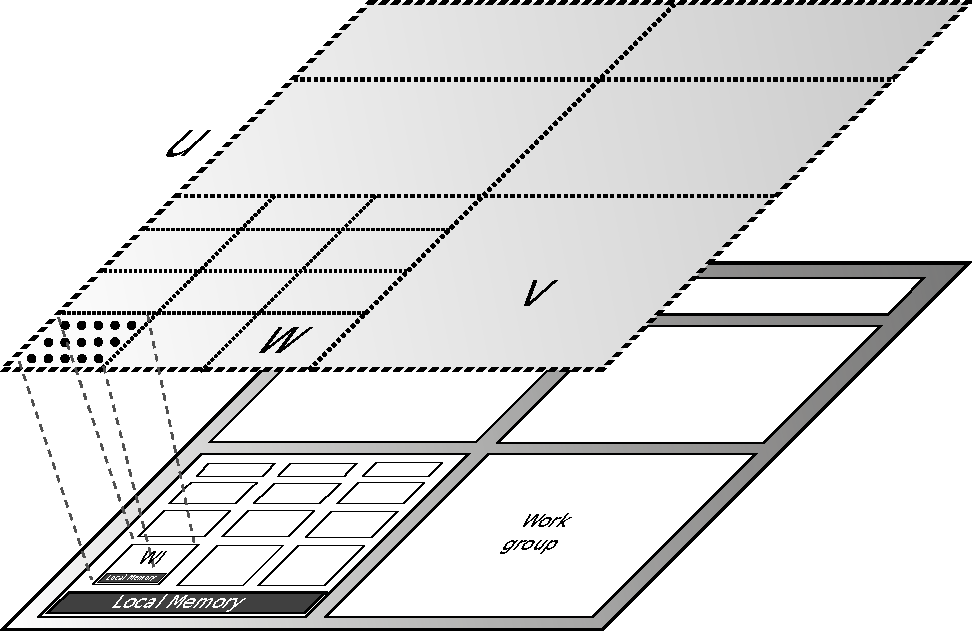
\includegraphics[width=0.8\columnwidth]{fig/archmapping.pdf}
	\caption{Mapping between data and hardware. Both hardware architecture (bottom layer) and data (top layer) are viewed
		hierarchically: the domain \texttt{u} is subdivided into \texttt{v} and \texttt{w}, the hardware architecture groups parallel execution
		units on multiple levels together.}
	\label{fig:hwmapping}
\end{figure}


\section{Examples of Generated Code}

To conclude this chapter, we show two examples how a simple strategy iterator is mapped to code,
once for a OpenMP-parallelized shared memory CPU system, and once for a CUDA-programmed NVIDIA GPU.

Listing \ref{lst:stg-generated-openmp} shows an example of a generated C code using OpenMP for parallelization.
It was generated for a 3D stencil from the parallel Strategy subdomain iterator
``\lstinline[language=strategy]!for subdomain v(cb) in u(:; t) parllel ...!''.
OpenMP provides one level of one-dimensional indexing (by the thread number, \texttt{omp\_get\_thread\_num ()}), but
the domain to decomposed is $3$-dimensional. Thus, the $3$-dimensional index range\index{index calculation}
\[
	[\mathtt{v\_idx\_x}, \mathtt{v\_idx\_x\_max}] \times
	[\mathtt{v\_idx\_y}, \mathtt{v\_idx\_y\_max}] \times [\mathtt{v\_idx\_z}, \mathtt{v\_idx\_z\_max}]
\]
is calculated based on the thread ID. By incrementing the loop index \texttt{v\_idx} by the number of threads,
the \texttt{v} blocks are dealt out cyclically.

\begin{lstlisting}[language=C, label=lst:stg-generated-openmp,
	caption={C/OpenMP code generated for a 3D stencil from the Strategy iterator
	``{\lstinline[language=strategy]!for subdomain v(cb) in u(:; t) parallel ...!}''.}]
int dimidx0 = omp_get_thread_num();
int dimsize0 = omp_get_num_threads();
int v_numblocks =
	((x_max+cb_x-1)/cb_x)*((y_max+cb_y-1)/cb_y)*((z_max+cb_z-1)/cb_z);
for (v_idx=dimidx0; v_idx <= v_numblocks-1; v_idx += dimsize0)
{
	tmp_stride_0z = ((x_max+cb_x-1)/cb_x)*((y_max+cb_y-1)/cb_y);
	v_idx_z = v_idx/tmp_stride_0z;
	tmpidxc0 = v_idx-(v_idx_z*tmp_stride_0z);
	v_idx_y = tmpidxc0/((x_max+cb_x-1)/cb_x);
	tmpidxc0 -= v_idx_y*((x_max+cb_x-1)/cb_x);
	v_idx_x = tmpidxc0;
	v_idx_x = v_idx_x*cb_x+1;
	v_idx_x_max = min(v_idx_x+cb_x, x_max+1);
	v_idx_y = v_idx_y*cb_y+1;
	v_idx_y_max = min(v_idx_y+cb_y, y_max+1);
	v_idx_z = v_idx_z*cb_z+1;
	v_idx_z_max = min(v_idx_z+cb_z, z_max+1);

	// inner loops/computation within [v_idx_x, v_idx_x_max] x ...
}
\end{lstlisting}

In contrast, CUDA provides $2$ levels of indexing, the thread block and the thread level.
Moreover, the indices on the thread block level can be $1$ or $2$-dimensional (prior to CUDA 4.0) or
$1$, $2$, or $3$-dimensional in CUDA 4.0 on a Fermi GPU, and thread indices
can be $1$, $2$, or $3$-dimensional.
Also, a GPU being a many-core architecture, we assume that there are enough threads to compute the
iterates in \texttt{v} completely in parallel. Hence, there is no loop iterating over the domain,
but a conditional guarding the ``iteration'' space instead as shown in Listing \ref{lst:stg-generated-cuda}.

\begin{lstlisting}[language=C, label=lst:stg-generated-cuda,
	caption={C for CUDA code generated for a 3D stencil from the Strategy iterator
	``{\lstinline[language=strategy]!for subdomain v(cbx, 1 ...) in u(:; t) parallel ...!}''.}]
stride_1 = (blockDim.y+y_max-1)/blockDim.y;
tmp = blockIdx.y;
idx_1_2 = tmp/stride_1;
tmp -= idx_1_2*stride_1;
idx_1_1 = tmp;
v_idx_x = 1+(blockDim.x*blockIdx.x+threadIdx.x)*cbx;
v_idx_x_max = v_idx_x+cbx;
v_idx_y = threadIdx.y+idx_1_1*blockDim.y+1;
v_idx_y_max = v_idx_y+1;
v_idx_z = threadIdx.z+idx_1_2*blockDim.z+1;
v_idx_z_max = v_idx_z+1;

if ((((v_idx_x<=x_max)&&(v_idx_y<=y_max))&&(v_idx_z<=z_max))) {
	// inner loops/computation within [v_idx_x, v_idx_x_max] x ...
}
\end{lstlisting}
Again, the $3$-dimensional index range
\[
	[\mathtt{v\_idx\_x}, \mathtt{v\_idx\_x\_max}] \times
	[\mathtt{v\_idx\_y}, \mathtt{v\_idx\_y\_max}] \times [\mathtt{v\_idx\_z}, \mathtt{v\_idx\_z\_max}]
\]
is calculated before the actual calculation, but now based on the $2$-dimensional thread block indices
\texttt{(blockIdx.x, blockIdx.y)} and the $3$-dimensional thread indices \texttt{(threadIdx.x, threadIdx.y, threadIdx.z)}.\\
\texttt{blockIdx} and \texttt{threadIdx} are built-in variables in C for CUDA.
